%source mathadata
On calcule une \textbf{caractéristique} $\color{red}{x}$ d'une image comme étant la moyenne des valeurs des pixels de l'image dans le rectangle rouge.
	\begin{MADenumerate}
		\item Calculer la caractéristique $\color{red}{x}$ pour chacune de ces quatre images.
		\begin{multicols*}{4}
			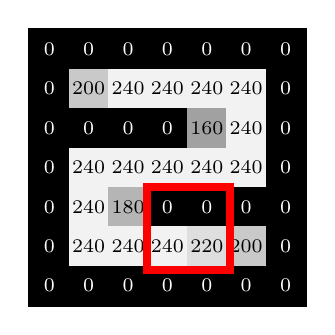
\begin{tikzpicture}[scale=0.5]
				\def\grid{
					{0,0,0,0,0,0,0},
					{0,200,240,240,240,240,0},
					{0,0,0,0,160,240,0},
					{0,240,240,240,240,240,0},
					{0,240,180,0,0,0,0},
					{0,240,240,240,220,200,0},
					{0,0,0,0,0,0,0},
				}                \foreach \row[count=\i from 0] in \grid {                \foreach \value[count=\j from 0] in \row {
						\pgfmathsetmacro{\gray}{int(100-\value/2.55)}
						\fill[black!\gray!white] (\j, -\i) rectangle ++(1, -1);
						\pgfmathsetmacro{\textcolor}{ifthenelse(\gray<50, "black", "white")}
						% réduire la taille : \small, \footnotesize, \scriptsize, \tiny
						\node[text=\textcolor] at (\j+0.5, -\i-0.5) {\scriptsize \value};                }
				}
				\draw[black, line width=0.5mm] (0, 0) rectangle (7, -7);
				\draw[red, line width=1mm] (2.99, -3.99) -- (5.1, -3.99)--(5.1,-6.1)--(2.99,-6.1)--cycle;
			\end{tikzpicture}
			\columnbreak

			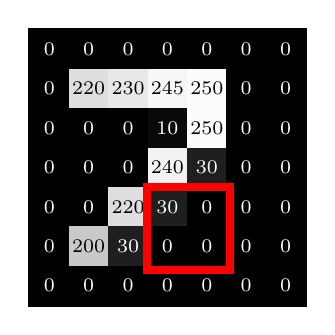
\begin{tikzpicture}[scale=0.5]
				\def\grid{
					{0,0,0,0,0,0,0},
					{0,220,230,245,250,0,0},
					{0,0,0,10,250,0,0},
					{0,0,0,240,30,0,0},
					{0,0,220,30,0,0,0},
					{0,200,30,0,0,0,0},
					{0,0,0,0,0,0,0},                }                \foreach \row[count=\i from 0] in \grid {                \foreach \value[count=\j from 0] in \row {
						\pgfmathsetmacro{\gray}{int(100-\value/2.55)}
						\fill[black!\gray!white] (\j, -\i) rectangle ++(1, -1);
						\pgfmathsetmacro{\textcolor}{ifthenelse(\gray<50, "black", "white")}
						\node[text=\textcolor] at (\j+0.5, -\i-0.5) {\scriptsize \value};
					}
				}
				\draw[black, line width=0.5mm] (0, 0) rectangle (7, -7);
				\draw[red, line width=1mm] (2.99, -3.99) -- (5.1, -3.99)--(5.1,-6.1)--(2.99,-6.1)--cycle;
			\end{tikzpicture}
			\columnbreak

			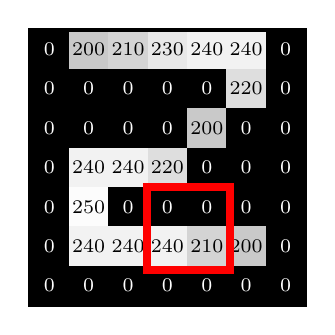
\begin{tikzpicture}[scale=0.5]
				\def\grid{
					{0,200,210,230,240,240,0},
					{0,0,0,0,0,220,0},
					{0,0,0,0,200,0,0},
					{0,240,240,220,0,0,0},
					{0,250,0,0,0,0,0},
					{0,240,240,240,210,200,0},
					{0,0,0,0,0,0,0},                }                \foreach \row[count=\i from 0] in \grid {                \foreach \value[count=\j from 0] in \row {                \pgfmathsetmacro{\gray}{int(100-\value/2.55)}
						\fill[black!\gray!white] (\j, -\i) rectangle ++(1, -1);
						\pgfmathsetmacro{\textcolor}{ifthenelse(\gray<50, "black", "white")}
						\node[text=\textcolor] at (\j+0.5, -\i-0.5) {\scriptsize \value};
					}
				}
				\draw[black, line width=0.5mm] (0, 0) rectangle (7, -7);
				\draw[red, line width=1mm] (2.99, -3.99) -- (5.1, -3.99)--(5.1,-6.1)--(2.99,-6.1)--cycle;
			\end{tikzpicture}
			\columnbreak 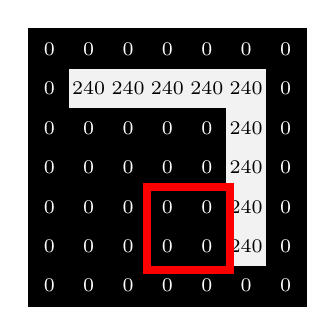
\begin{tikzpicture}[scale=0.5] \def\grid{
					{0,0,0,0,0,0,0},
					{0,240,240,240,240,240,0},
					{0,0,0,0,0,240,0},
					{0,0,0,0,0,240,0},
					{0,0,0,0,0,240,0},
					{0,0,0,0,0,240,0},
					{0,0,0,0,0,0,0}, } \foreach \row[count=\i from 0] in \grid { \foreach \value[count=\j from 0] in \row { \pgfmathsetmacro{\gray}{int(100-\value/2.55)} \fill[black!\gray!white] (\j, -\i) rectangle ++(1, -1); \pgfmathsetmacro{\textcolor}{ifthenelse(\gray<50, "black", "white")} \node[text=\textcolor] at (\j+0.5, -\i-0.5) {\scriptsize \value}; } }
				\draw[black, line width=0.5mm] (0, 0) rectangle (7, -7);
				\draw[red, line width=1mm] (2.99, -3.99) -- (5.1, -3.99)--(5.1,-6.1)--(2.99,-6.1)--cycle; \end{tikzpicture}

		\end{multicols*}

		\item  Le tableau suivant donne les valeurs de la caractéristique $\color{red}x$ d'une liste d'images d'entraînement dont on connaît le chiffre (2 ou 7).
		\begin{center}
			\hspace{-1.4cm}
			\begin{tabular}{|c|*{5}{>{\columncolor{BleuCeladon!20}}c|}*{5}{>{\columncolor{OrangeCarotte!20}}c|}}
				\hline
				\rowcolor{floralwhite}Image
				                 & \includegraphics[width=.05\linewidth]{images/image_2_rec_1.jpg}
				                 & \includegraphics[width=.05\linewidth]{images/image_2_rec_2.jpg}
				                 & \includegraphics[width=.05\linewidth]{images/image_2_rec_3.jpg}
				                 & \includegraphics[width=.05\linewidth]{images/image_2_rec_4.jpg}
				                 & \includegraphics[width=.05\linewidth]{images/image_2_rec_5.jpg}
				                 & \includegraphics[width=.05\linewidth]{images/image_7_rec_1.jpg}
				                 & \includegraphics[width=.05\linewidth]{images/image_7_rec_2.jpg}
				                 & \includegraphics[width=.05\linewidth]{images/image_7_rec_3.jpg}
				                 & \includegraphics[width=.05\linewidth]{images/image_7_rec_4.jpg}
				                 & \includegraphics[width=.05\linewidth]{images/image_7_rec_5.jpg}                                                \\\hline

				Chiffre          & 2                                                               & 2   & 2   & 2   & 2   & 7   & 7 & 7 & 7 & 7  \\\hline
				$\color{red}{x}$ & 150                                                             & 230 & 190 & 100 & 162 & 160 & 5 & 7 & 0 & 80 \\\hline
			\end{tabular}
		\end{center}
		Si une nouvelle image a la caractéristique $\color{red}{x}$ $=20$, à quel chiffre correspond-elle ? Justifier la réponse.
		\item \begin{multicols}{2}
			Voici un algorithme qui utilise la caractéristique $x$ pour différencier les images de 2 et de 7. Pour que l'algorithme (I) commette le moins d'erreurs possible sur les images du tableau, attribuer à $a$ et $b$ les valeurs 2 ou 7 et justifier ce choix.

			\begin{center}

				\begin{tabular}{|lcll|}
					\hline
					Entrée       &  & \multicolumn{2}{l|}{Image numérique}                                \\

					Instructions &  & \multicolumn{2}{l|}{Calcul de la valeur de $x$}                     \\
					             &  & \multicolumn{2}{l|}{Si $\color{red}{x}$ $<10$, alors}               \\
					             &  & \multicolumn{1}{l}{$\quad$}                           & Réponse = a \\
					             &  & \multicolumn{2}{l|}{Sinon}                                          \\
					             &  & \multicolumn{1}{l}{$\quad$}                           & Réponse = b \\
					             &  & \multicolumn{2}{l|}{Fin Si}                                         \\
					Sortie       &  & \multicolumn{2}{l|}{Afficher Réponse}                               \\\hline\end{tabular}

				Algorithme (I)\\ \end{center}

		\end{multicols}

		\item Calculer le pourcentage d'erreur de cet algorithme appliqué aux images du tableau.
		\item Modifier la ligne \textit{"Si $\color{red}{x} $ $<10$, alors"} pour réduire le pourcentage d'erreur de l'algorithme sur les images d'entraînement du tableau et calculer le pourcentage d'erreur obtenu.
	\end{MADenumerate}
